\begin{center}
    {\LARGE \textbf{2019无机化学}} \\[2ex]
    {\large 时量180分钟 \quad 满分100分}
\end{center}

\vspace{0.5cm}
\noindent\textbf{注意事项:}
\begin{enumerate}[label=\arabic*., parsep=0pt, itemsep=0pt]
    \item 答题前,考生先将自己的姓名、学号、考场号、座位号填写在答题卡上,将条形码准确粘贴在考生信息条形码粘贴区。
    \item 考试结束后,将本试卷与答题纸一并收回。
    \item 回答各个问题时,将答案写在答题纸上,写在本试卷上无效。
\end{enumerate}

\vspace{0.5cm}
\noindent\textbf{一、选择题(20 pts.)}

\begin{enumerate}[label=\arabic*., itemsep=1.5ex]
    \item 往$\ce{FeCl3}$溶液中加入少量$\ce{KI}$，反应的结果是
    \begin{tasks}(4)
        \task 有$\ce{I2}$单质析出
        \task 生成$\ce{IO3^-}$
        \task 生成$\ce{FeI3}$
        \task 生成$\ce{I3^-}$
    \end{tasks}
    \item 下列配合物中，肯定有颜色的是
    \begin{tasks}(4)
        \task $\ce{[CuCl2]^-}$
        \task $\ce{[Ag(S2O3)2]^3-}$
        \task $\ce{[Ni(NH3)6]^2+}$
        \task $\ce{[Cd(NH3)4]^2+}$
    \end{tasks}
    \item 下列物质中碱性最强的是
    \begin{tasks}(4)
        \task $\ce{Sn(OH)2}$
        \task $\ce{Sn(OH)4}$
        \task $\ce{Ge(OH)2}$
        \task $\ce{Ge(OH)4}$
    \end{tasks}
    \item 下列配离子中,能够将$\ce{KI}$氧化的是
    \begin{tasks}(4)
        \task $\ce{[Fe(CN)6]^3-}$
        \task $\ce{[Fe(SCN)6]^3-}$
        \task $\ce{[Co(NH3)6]^3+}$
        \task $\ce{[Ni(CN)6]^2-}$
    \end{tasks}
    \item 在酸性介质中可将$\ce{Cr^3+}$氧化为$\ce{Cr2O7^2-}$的试剂是
    \begin{tasks}(4)
        \task 王水
        \task $\ce{PbO2}$
        \task $\ce{MnO2}$
        \task $\ce{H2O2}$
    \end{tasks}
    \item 将$\ce{SiF4}$通入$\ce{NaOH}$溶液中，主要产物是
    \begin{tasks}(4)
        \task $\ce{H4SiO4 + NaF}$
        \task $\ce{Na2SiO3 + NaF}$
        \task $\ce{Na2SiO3 + Na2SiF6}$
        \task $\ce{SiO2 + HF}$
    \end{tasks}
    \item 将$\ce{NCl3}$通入$\ce{NaOH}$溶液，得到的产物是
    \begin{tasks}(4)
        \task $\ce{NH3}$和$\ce{NaCl}$
        \task $\ce{NH3}$和$\ce{NaClO}$
        \task $\ce{NO2}$和$\ce{NaCl}$
        \task $\ce{NH4Cl}$
    \end{tasks}
    \item 下列溶液，长期暴露于空气中会变颜色的是
    \begin{tasks}(4)
        \task $\ce{Na2S}$
        \task $\ce{Na2SO4}$
        \task $\ce{K2S2O8}$
        \task $\ce{Na2O2}$
    \end{tasks}
    \item 下列各对元素中，性质差异最大的是
    \begin{tasks}(4)
        \task $\ce{Nb}$和$\ce{Ta}$
        \task $\ce{Ti}$和$\ce{V}$
        \task $\ce{Zr}$和$\ce{Hf}$
        \task $\ce{Mo}$和$\ce{W}$
    \end{tasks}
    \item 按分子轨道理论，下列分子或离子中最不稳定的是
    \begin{tasks}(4)
        \task $\ce{N2}$
        \task $\ce{N2^+}$
        \task $\ce{N2^-}$
        \task $\ce{N2^2-}$
    \end{tasks}
\end{enumerate}

\vspace{0.5cm}
\noindent\textbf{二、写出实验现象并给出相关反应方程式（40 pts.）}

\begin{enumerate}[label=\arabic*., start=1, itemsep=1.5ex]
    \item 向酸性$\ce{Cr2O7^2-}$溶液中加入金属锌。
    \item 分别向$\ce{[Cu(NH3)4]SO4}$溶液中缓慢添加稀硫酸和快速添加稀硫酸。
    \item 向$\ce{Fe2(SO4)3}$溶液中依次加入饱和$\ce{(NH4)2C2O4}$溶液、少量$\ce{KSCN}$溶液、少量盐酸和过量$\ce{NH4F}$溶液。
    \item 向$\ce{KI}$溶液中滴加双氧水。
    \item 向$\ce{[CuCl4]^2-}$溶液中滴加$\ce{KI}$溶液。再加入适量的$\ce{Na2SO3}$溶液。
    \item 向$\ce{K2MnO4}$溶液中缓慢通入$\ce{NO2}$。
    \item 向$\ce{NiSO4}$溶液中缓通入稀氨水。
    \item 向$\ce{Hg^{2+}}$溶液中加入$\ce{KI}$溶液。
    \item 将$\ce{BiCl3}$溶液和$\ce{NaOH}$溶液充分混合，再向其中通入氧气。
    \item 在煤气灯上加热$\ce{Cu(NO3)2\cdot 2H2O}$晶体。
\end{enumerate}

\vspace{0.5cm}
\noindent\textbf{三、简答题（40 pts.）}

\begin{enumerate}[label=\arabic*., start=1, itemsep=1.5ex]
    \item $\ce{Cu}$、$\ce{Zn}$在元素周期表中同属$\ce{ds}$区且相邻，实验测得$\ce{Cu}$的第一电离能为$746\,\mathrm{kJ\cdot mol^{-1}}$，而$\ce{Zn}$的第一电离能为$906\,\mathrm{kJ\cdot mol^{-1}}$，从电离能数据看，$\ce{Cu}$应比$\ce{Zn}$活泼，但事实上，$\ce{Zn}$的活泼性远强于$\ce{Cu}$，试解释原因。
    \item 在标准状态下，$\ce{Co(III)}$能将水氧化，通过计算说明在$1\,\mathrm{mol\cdot dm^{-3}}$的$\ce{NH3}$溶液中，$\ce{Co(III)}$能否将水氧化，已知：$E^\ominus(\ce{Co^{3+}/Co^{2+}})=1.84V$，$E^\ominus(\ce{O2/H2O})=1.23V$，$K^\ominus_{\text{稳}}[\ce{Co(NH3)4}]^{3+}=2\times10^{35}$，$K^\ominus_{\text{稳}}[\ce{Co(NH3)6}]^{2+}=1.3\times10^{5}$
    \item 比较下列各对配合物的稳定性，并简要说明原因。
    \begin{enumerate}[label=(\arabic*), itemsep=1ex]
        \item $\ce{[Ag(NH3)2]^+}$与$\ce{[Ag(S2O3)2]^3-}$
        \item $\ce{[Co(NH3)6]^2+}$与$\ce{[Co(NH3)6]^3+}$
        \item $\ce{[Cu(NH3)4]^2+}$与$\ce{[Cu(en)2]^2+}$
        \item $\ce{[HgI2]^2-}$与$\ce{[HgCl4]^2-}$
        \item $\ce{[Cu(NH3)4]^2+}$与$\ce{[Zn(NH3)4]^2+}$
    \end{enumerate}
    \item 请解释：$\ce{[Co(NH3)6]^3+}$的稳定常数是$\ce{[Co(NH3)6]^2+}$的$10$倍，而$\ce{[Fe(CN)6]^3-}$的稳定常数仅是$\ce{[Fe(CN)6]^4-}$的$10^7$倍。
    \item 给出$\ce{BCl3}$和$\ce{BF3}$的水解反应方程式，解释为什么二者水解产物不同？
    \item 为什么$\ce{SnS2}$溶于$\ce{Na2S}$溶液；而$\ce{SnS}$不溶于$\ce{Na2S}$溶液但溶于$\ce{Na2S2}$溶液。
    \item 试比较$\ce{NH3}$、$\ce{N2H4}$、$\ce{NH2OH}$、$\ce{HN3}$碱性强弱并说明原因。
    \item 请解释：
    \begin{enumerate}[label=(\arabic*), itemsep=1ex]
        \item 由$\ce{CoCl2}$与饱和$\ce{KNO2}$溶液制备$\ce{K3[Co(NO2)6]}$时，需加入醋酸酸化。
        \item 用浓盐酸处理$\ce{Co2O3}$得到蓝色溶液，加水稀释后溶液变为粉红色。
        \item 向盛$\ce{Na2S2O3}$溶液的试管中加$1$滴$\ce{AgNO3}$溶液，生成白色沉淀，摇动试管则沉淀立即溶解；向盛$\ce{AgNO3}$溶液的试管中加$1$滴$\ce{Na2S2O3}$溶液，生成白色沉淀，摇动试管沉淀不溶解。
    \end{enumerate}
\end{enumerate}

\vspace{0.5cm}
\noindent\textbf{四、制备与分离（20 pts.）}

\begin{enumerate}[label=\arabic*., start=1, itemsep=1.5ex]
    \item 如何用化学方法除去下列物质中的少量杂质？给出相关的反应方程式
    \begin{enumerate}[label=(\arabic*), itemsep=1ex]
        \item $\ce{CO2}$气体中的少量$\ce{SO2}$杂质；
        \item 金属银中少量的金属铜杂质；
        \item $\ce{CO2}$气体中的少量$\ce{O2}$杂质。
    \end{enumerate}
    \item 用化学法由软锰矿制各$\ce{KMnO4}$。
    \item 实验室中制取少量$\ce{HBr}$采用的方法是将红磷与水合后滴加液溴，为什么不能将红磷和液溴混合后滴加水制备$\ce{HBr}$？
    \item 设计方案分离含有$\ce{Cu^{2+}}$、$\ce{Zn^{2+}}$、$\ce{Hg^{2+}}$、$\ce{Al^3+}$、$\ce{Sn^{2+}}$的混合溶液。
\end{enumerate}

\vspace{0.5cm}
\noindent\textbf{五、鉴别与推断（30 pts.）}

\begin{enumerate}[label=\arabic*., start=1, itemsep=1.5ex]
    \item 3种无色溶液分别为$\ce{Na2S2O3}$、$\ce{Na2SO4}$、$\ce{Na2S2O4}$试加以鉴别。
    \item 有一种白色固体，可能是$\ce{SnCl2}$、$\ce{SiO2}$、$\ce{Pb(NO3)2}$、$\ce{PbCl2}$中的一种，由下列实验判断。该白色固体是哪种化合物？写出有关方程式。
    \begin{enumerate}[label=\arabic*), itemsep=1ex]
        \item 白色固体溶于盐酸；
        \item 白色固体能使碘-淀粉溶液褪色；
        \item 白色固体的盐酸溶液中加$\ce{H2O2}$，充分反应后通入$\ce{H2S}$，有黄色沉淀生成。
    \end{enumerate}
    \item 一黄色固体，可能是$\ce{PbCrO4}$、$\ce{BaCrO4}$、$\ce{SrO4}$，试加以鉴别并给出相关反应方程式。
    \item 相关化合物的转化关系如图所示，请写出$A-E$各物质的化学式。并写出$B\rightarrow C$的相关方程式。
   
    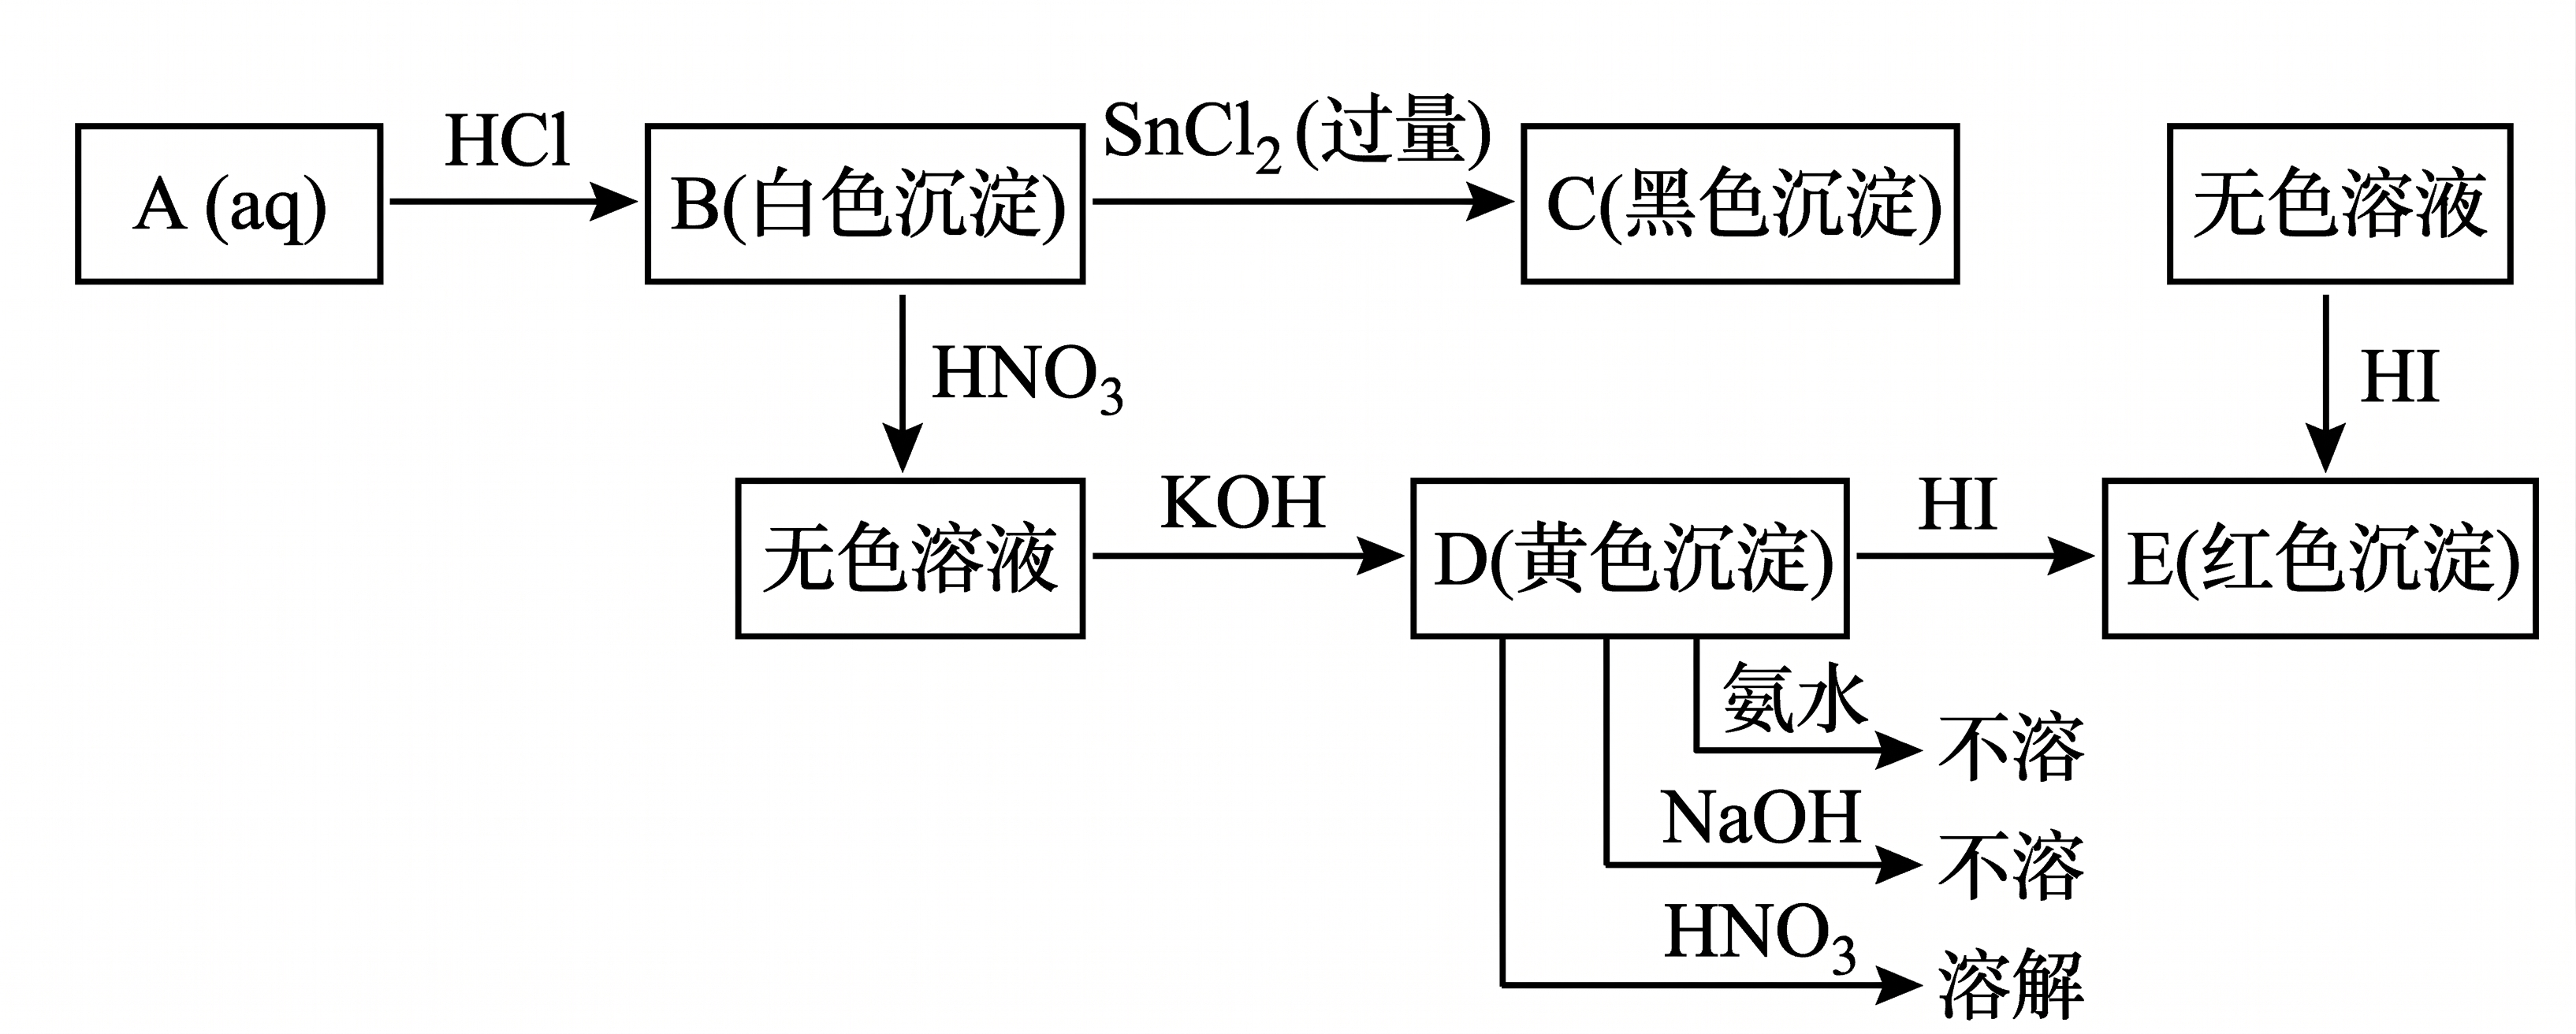
\includegraphics[width=0.5\textwidth]{2019_5_4}

    \item 绿色化合物$A$溶于稀硫酸生成$B$的溶液，无水盐$B$为棕红色。$A$也可溶于$\ce{KOH}$生成$C$的绿色溶液，向其中加入过氧化氢后呈黄色，说明变成了$D$的溶液，再向其中加入过量稀硫酸,溶液变橙色,因为$D$变成了$E$，继续加入戊醇和少量过氧化氢，震荡后在有机层中生成蓝色化合物$F$，将固体化合物$E$溶入到浓硫酸中，析出红色的针状结晶$G$。向$D$的溶液中加入硝酸银时生成砖红色沉淀$H$，试给出$A$,$E$,$F$,$G$的化学式，并完成$A\rightarrow B$、$E\rightarrow F$、$E\rightarrow G$的化学反应方程式。
    \item 绿色水合盐$A$在一定温度下脱水得到白色固体$B$，$B$在更高的温度下分解生成砖红色固体$C$和无色气体$D$，$D$与$\ce{Cl2}$在干燥的条件下经活性炭催化反应生成无水发烟液体$E$。向$C$的盐酸溶液中加入$\ce{NaOH}$生成棕色沉淀$F$，若向$C$的盐酸溶液中加入$\ce{K2C2O4}$并加热则得到黄色溶液，经蒸发、浓缩、冷却后，析出绿色水合晶体$G$。试给出$A$、$C$、$E$、$G$的化学式，并写出$B\rightarrow C$和$D\rightarrow E$的反应方程式。
\end{enumerate}